\documentclass[compress,svgnames,xcolor=table]{beamer}
\mode<presentation>

% Include additional LaTeX packages
\usepackage{etex}
\usepackage{pifont}
\usepackage{multicol}
\usepackage{amsmath}
\usepackage{epsfig}
\usepackage{pgfplots}
\usepackage{graphicx}
\usepackage[all,knot]{xy}
\xyoption{arc}
\usepackage{url}
\usepackage{multimedia}
\usepackage{hyperref}
\usepackage{setspace}
\usepackage{listings}
\usepackage{tikz}
\usetikzlibrary{positioning}
\usepackage{threeparttable}

\definecolor{lightgray}{gray}{.95}
\definecolor{darkgray}{gray}{.80}

% Set up Beamer theme
\usetheme{Dresden}
\usecolortheme{lily}
\usefonttheme{structuresmallcapsserif}
\usepackage{beamerinnerthemecircles}
\usepackage{beamerouterthememiniframes}
\useoutertheme[subsection=false]{smoothbars}

% Removes the Beamer navigation symbols
\setbeamertemplate{navigation symbols}{}

% Sets the color for the \alert{} text
\setbeamercolor{alerted text}{fg=blue}

% Presentation information
\title[RAISE 2012 -- \insertframenumber/\inserttotalframenumber]{Predicting Mutation Score Using Source Code and Test Suite Metrics \vspace{2mm} \hrule}
\subtitle{RAISE 2012}
\author[\copyright 2012, Kevin Jalbert and Jeremy S. Bradbury]{\textbf{Kevin Jalbert} and Jeremy S. Bradbury \\ \vspace{4mm} \scriptsize{\texttt{\{kevin.jalbert,jeremy.bradbury\}@uoit.ca}}}
\institute[UOIT]{Software Quality Research Group (\url{sqrg.ca})\\University of Ontario Institute of Technology\\Oshawa, Ontario, Canada}
\date{\tiny June 5$^{th}$, 2012}

\begin{document}

% Create title page
\frame{\maketitle}

\section{Overview}
\frame{
  \setcounter{tocdepth}{2}
  \tableofcontents[currentsection,hideothersubsections]
}

\subsection{Mutation Testing}
\frame{\frametitle{Mutation Testing}
  \centering
  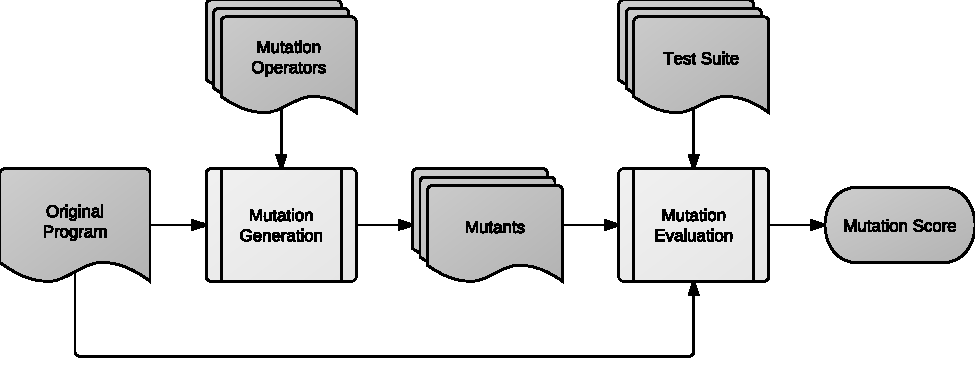
\includegraphics[width=8cm]{figures/mutation_testing_overview.pdf}
  \vspace{2mm}
  \begin{itemize}
    \item Create \alert{mutants} from original program using \alert{mutation operators}
    \item Compare mutant's \alert{results} against original program using \alert{test suite}
    \item Mutation score is \alert{percent} of non-equivalent mutants \alert{killed}
  \end{itemize}
}

\subsubsection{Mutation Operators}
\frame{\frametitle{Mutation Operators}
  \begin{table}[h]
    \centering
    \rowcolors{2}{gray!30}{gray!20}
    \begin{tabular}{|l|l|}
      \hline
      \rowcolor[RGB]{169,196,223}
      \textbf{Name} & \textbf{Description} \\
      \hline REPLACE\_CONSTANT & Replace a constant \\
      \hline NEGATE\_JUMP & Negate jump condition \\
      \hline ARITHMETIC\_REPLACE & Replace arithmetic operator \\
      \hline REMOVE\_CALL & Remove method call \\
      \hline REPLACE\_VARIABLE & Replace variable reference\\
      \hline ABSOLUTE\_VALUE & Insert absolute value of a variable \\
      \hline UNARY\_OPERATOR & Insert unary operator \\
      \hline
    \end{tabular}
  \end{table}
}

\subsubsection{Mutation Operators}
\frame{\frametitle{Mutation Operators}
  \begin{table}[h]
    \centering
    \rowcolors{2}{gray!30}{gray!20}
    \begin{tabular}{|l|l|}
      \hline
      \rowcolor[RGB]{169,196,223}
      \textbf{Name} & \textbf{Description} \\
      \hline REPLACE\_CONSTANT & Replace a constant \\
      \hline NEGATE\_JUMP & Negate jump condition \\
      \rowcolor[RGB]{169,166,223}
      \hline ARITHMETIC\_REPLACE & Replace arithmetic operator \\
      \hline REMOVE\_CALL & Remove method call \\
      \hline REPLACE\_VARIABLE & Replace variable reference\\
      \hline ABSOLUTE\_VALUE & Insert absolute value of a variable \\
      \hline UNARY\_OPERATOR & Insert unary operator \\
      \hline
    \end{tabular}
  \end{table}
}

\subsubsection{Example Operator -- ARITHMETIC\_REPLACE}
\frame{\frametitle{Example Operator -- ARITHMETIC\_REPLACE}
  \begin{figure}
    \centering
    \begin{minipage}{5.5cm}
    \centering
    \footnotesize{\textbf{Correct Program}}
    \tiny
    \lstinputlisting[language=Java, literate={++this.current}{{\textcolor{red}{$++$\textbf{this}.current}}}{10}]{listings/mutation_example.java}
    \end{minipage}
    \vspace{4mm}
    \hrule
    \vspace{4mm}
    \begin{minipage}{5.5cm}
    \centering
    \footnotesize{\textbf{Mutant Program}}
    \tiny
    \lstinputlisting[language=Java, literate={++this.current}{{\textcolor{red}{$--$\textbf{this}.current}}}{10}]{listings/mutation_example.java}
    \end{minipage}
  \end{figure}
}

\subsection{Problem}
\frame{\frametitle{Problem}
  \begin{itemize}
    \item Mutation testing is an \alert{effective} yet \alert{costly} coverage technique
      \begin{itemize}
        \item A \alert{fault}-based \alert{coverage} technique
        \item Closest measure to \alert{test suite effectiveness}
      \end{itemize}
    \item Mutation testing would have to be applied \alert{frequently} during development
  \end{itemize}
}

\subsection{Our Solution}
\frame{\frametitle{Our Solution}
  \begin{quote}
  \Large
  \centering
    ``Our proposed approach uses machine learning to predict the mutation score based on a combination of source code and test suite metrics of the code unit under test''
  \end{quote}
  \vspace{5mm}
  \hrule
  \vspace{5mm}
  \begin{itemize}
    \item A \alert{``do fewer and smarter''} technique for mutation testing
    \begin{itemize}
      \item Identify source code units that have \alert{low/high coverage}
      \item Ability to \alert{prioritize} mutation testing for specific mutants
    \end{itemize}
  \end{itemize}
}

\subsection{Our Approach}
\frame{\frametitle{Our Approach}
  \begin{itemize}
    \item Collect \alert{feature data} for source code units
    \begin{itemize}
      \item Source code metrics
      \item Test suite metrics
    \end{itemize}
    \item Collect \alert{category data} for source code units
      \begin{itemize}
        \item Mutation score for source code units
      \end{itemize}
    \item \alert{Train} and \alert{predict} class and method source code units using a Support Vector Machine (SVM)
  \end{itemize}
}

\section{Background}
\frame{
  \setcounter{tocdepth}{2}
  \tableofcontents[currentsection,hideothersubsections]
}

\subsection{Support Vector Machine}
\frame{\frametitle{Support Vector Machine}
  \begin{itemize}
    \item A \alert{supervised} machine learning \alert{classification} technique
    \item Models a \alert{feature space} constructed using a \alert{set of vectors}
    \item Each \alert{vectors} has a set of \alert{attributes} and a \alert{category}
    \item Attempts to \alert{linearly separate} vectors
  \end{itemize}
  \begin{figure}
    \centering
    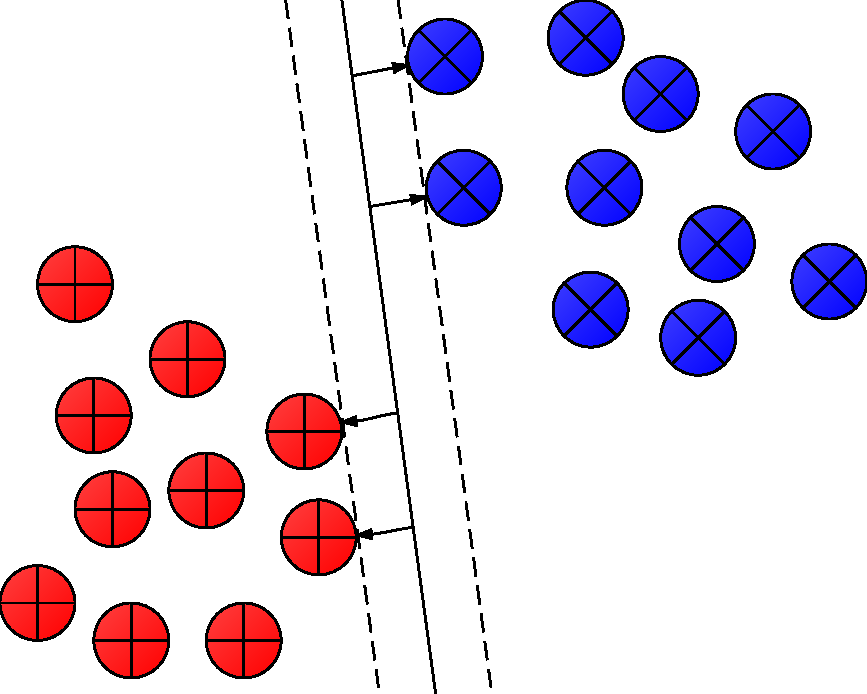
\includegraphics[width=3.5cm]{figures/SVM_small_margin.pdf}
    $\xrightarrow{\texttt{Better Margin}}$
    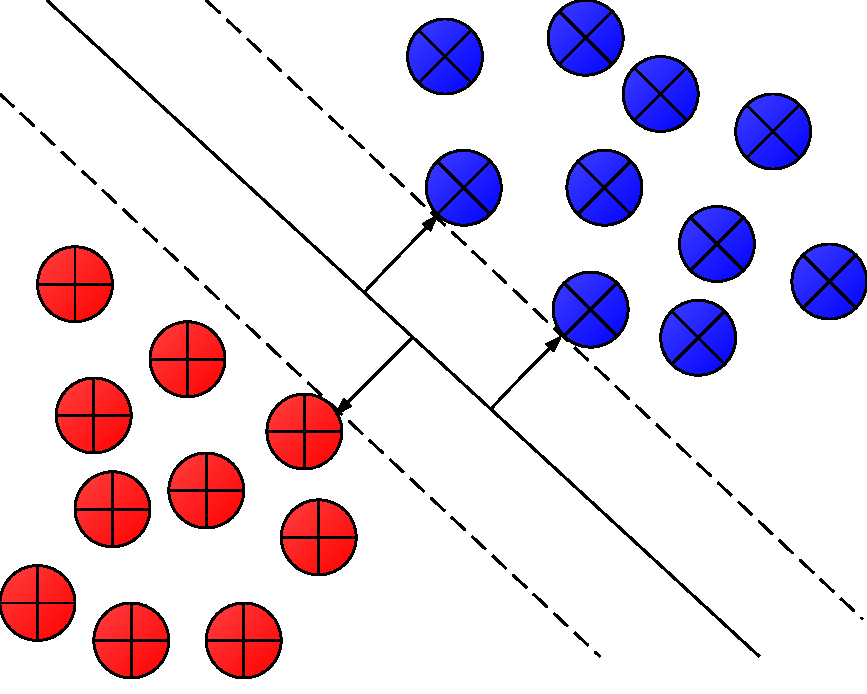
\includegraphics[width=3.5cm]{figures/SVM_maximum_margin.pdf}
  \end{figure}
}

\subsubsection{Support Vector Machine -- cont.}
\frame{\frametitle{Support Vector Machine -- cont.}
  \begin{itemize}
    \item Can work for \alert{\emph{many}-group} classification
    \item Can work on \alert{non-linearly separable} data using \alert{kernel functions}
  \end{itemize}
  \begin{figure}
    \centering
    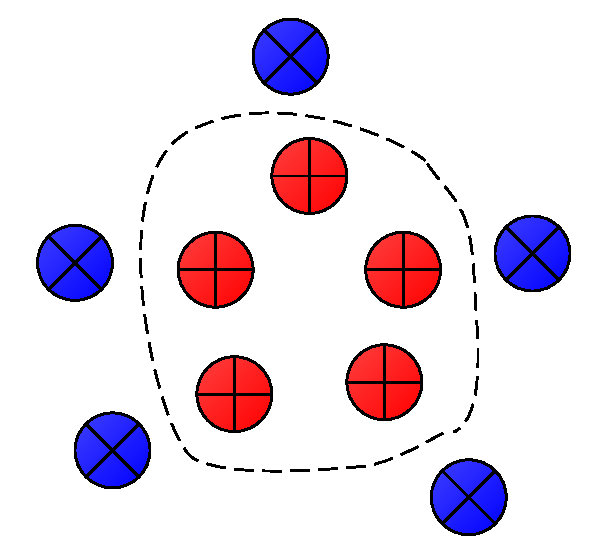
\includegraphics[width=3.5cm]{figures/SVM_non-linear.pdf}
    $\xrightarrow{\texttt{Kernel Function}}$
    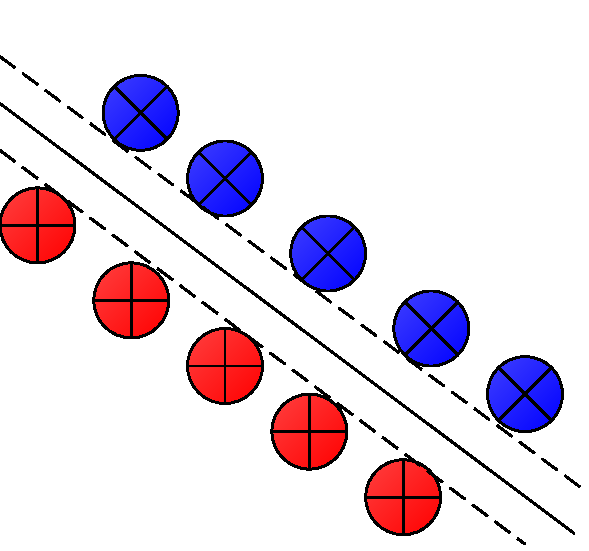
\includegraphics[width=3.5cm]{figures/SVM_kernel_function.pdf}
  \end{figure}
}

\subsection{Metrics}
\frame{\frametitle{Metrics}
  \begin{itemize}
    \item \alert{Measurements} that describe \alert{structural} and \alert{behavioral} \alert{properties} of a software system -- We believe these properties \alert{affect} the \alert{mutation score} of source code units
    \item The \alert{combination} of \alert{source code} and \alert{test metrics} is fairly unique to our research.
  \end{itemize}
}

\section{Process}
\frame{
  \setcounter{tocdepth}{2}
  \tableofcontents[currentsection,hideothersubsections]
}

\subsection{Data Collection}
\frame{\frametitle{Data Collection}
  \begin{figure}
    \begin{minipage}{5.25cm}
      \begin{itemize}
        \item \alert{Input}: Units of test cases and units of source code
        \begin{enumerate}
          \item Collect \alert{mutation scores} using \texttt{Javalanche}\footnote{\tiny{\url{github.com/david-schuler/javalanche}}}
          \item Collect \alert{source code metrics} using \texttt{Eclipse Metrics Plugin}\footnote{\tiny{\url{metrics2.sourceforge.net/}}}
          \item Collect \alert{coverage metrics} using \texttt{EMMA}\footnote{\tiny{\url{emma.sourceforge.net/}}}
        \end{enumerate}
      \end{itemize}
    \end{minipage}
    \hfill
    \begin{minipage}{5.25cm}
      \flushright
      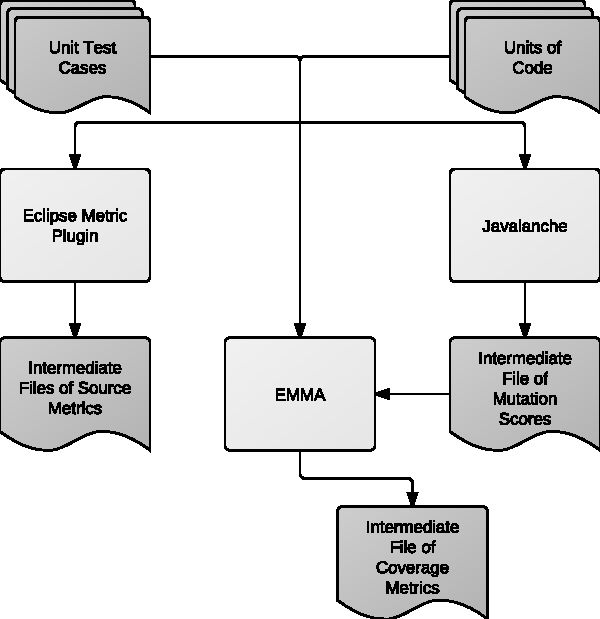
\includegraphics[width=5.25cm]{figures/process_part1.pdf}
      \vspace{-5mm}
      \Huge \centering
      \ldots
    \end{minipage}
  \end{figure}
}

\subsubsection{Source Code Metrics -- Methods}
\frame{\frametitle{Source Code Metrics -- Methods}
  \begin{table}
    \small
    \centering
    \rowcolors{2}{gray!30}{gray!20}
    \begin{tabular}{|l|l|}
      \hline
      \rowcolor[RGB]{169,196,223}
      \textbf{Description} & \textbf{Scope} \\
      \hline Method lines of code & Method \\
      \hline Nested block depth & Method \\
      \hline McCabe cyclomatic complexity & Method \\
      \hline Number of parameters & Method \\
      \hline
    \end{tabular}
  \end{table}
}

\subsubsection{Source Code Metrics -- Classes}
\frame{\frametitle{Source Code Metrics -- Classes}
  \begin{table}
    \small
    \centering
    \rowcolors{2}{gray!30}{gray!20}
    \begin{tabular}{|l|l|}
      \hline
      \rowcolor[RGB]{169,196,223}
      \textbf{Description} & \textbf{Scope} \\
      \hline Number of overridden methods & Class \\
      \hline Number of attributes & Class \\
      \hline Number of children & Class \\
      \hline Depth of inheritance tree & Class \\
      \hline Lack of cohesion of methods & Class \\
      \hline Number of static methods & Class \\
      \hline Number of methods & Class \\
      \hline Specialization index & Class \\
      \hline Weighted method per class & Class \\
      \hline Number of static attributes & Class \\
      \hline
    \end{tabular}
  \end{table}
}

\subsubsection{Test Code Metrics -- Coverage}
\frame{\frametitle{Test Code Metrics -- Coverage}
  \begin{table}
    \small
    \centering
    \rowcolors{2}{gray!30}{gray!20}
    \begin{tabular}{|l|l|}
      \hline
      \rowcolor[RGB]{169,196,223}
      \textbf{Description} & \textbf{Scope} \\
      \hline Basic blocks covered in code unit & Class/Method \\
      \hline Total basic blocks for code unit & Class/Method \\
      \hline
    \end{tabular}
  \end{table}
}

\subsubsection{Data Collection [recap.]}
\frame{\frametitle{Data Collection [recap.]}
  \begin{figure}
    \begin{minipage}{5.25cm}
      \begin{itemize}
        \item \alert{Input}: Units of test cases and units of source code
        \begin{enumerate}
          \item Collect \alert{mutation scores} using \texttt{Javalanche}\footnote{\tiny{\url{github.com/david-schuler/javalanche}}}
          \item Collect \alert{source code metrics} using \texttt{Eclipse Metrics Plugin}\footnote{\tiny{\url{metrics2.sourceforge.net/}}}
          \item Collect \alert{coverage metrics} using \texttt{EMMA}\footnote{\tiny{\url{emma.sourceforge.net/}}}
        \end{enumerate}
      \end{itemize}
    \end{minipage}
    \hfill
    \begin{minipage}{5.25cm}
      \flushright
      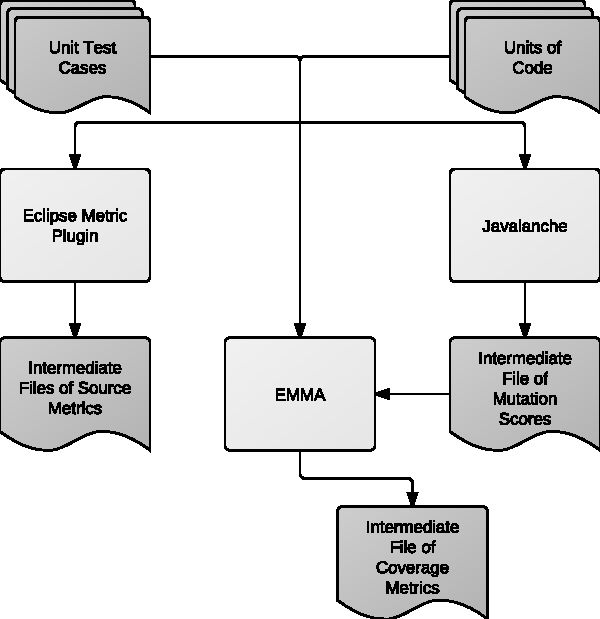
\includegraphics[width=5.25cm]{figures/process_part1.pdf}
      \vspace{-5mm}
      \Huge \centering
      \ldots
    \end{minipage}
  \end{figure}
}

\subsection{Data Synthesis}
\frame{\frametitle{Data Synthesis}
  \begin{figure}
    \begin{minipage}{5.25cm}
      \begin{itemize}
        \item \alert{Goal}: Category/feature data for source code units
        \begin{enumerate}
          \item \alert{Combine} source code and coverage metrics together
          \item \alert{Merge} source code metrics of the \alert{touched tests} for each source code unit
          \item \alert{Aggregate method-level} source code unit metrics into \alert{class-level} source code units
          \item \alert{Create \texttt{.libsvm}} file using feature/category data
        \end{enumerate}
      \end{itemize}
    \end{minipage}
    \hfill
    \begin{minipage}{5.25cm}
      \Huge \centering
      \ldots
      \vspace{-2mm}
      \flushright
      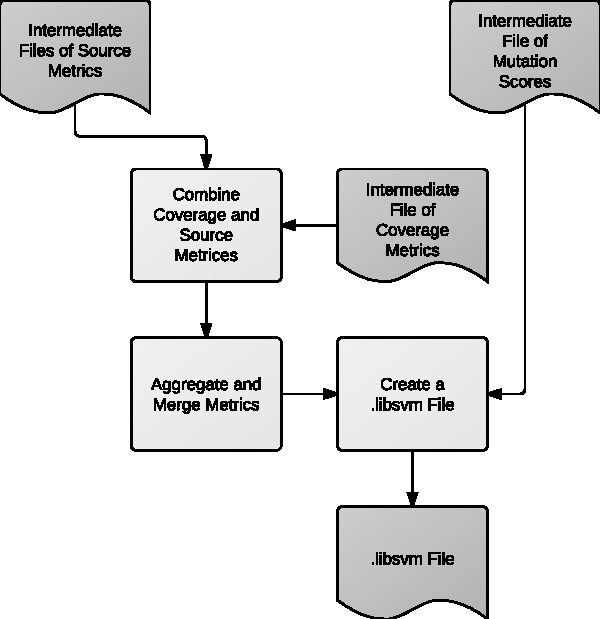
\includegraphics[width=5.25cm]{figures/process_part2.pdf}
    \end{minipage}
  \end{figure}
}

\subsubsection{Test Code Metrics -- Accumulated Tests}
\frame{\frametitle{Test Code Metrics -- Accumulated Tests}
  \begin{itemize}
    \item Each source code unit has a set of \alert{associated test cases} that \alert{touch the unit} during test execution.
    \item We can acquire the \alert{summation} and \alert{average} of the \alert{associated test cases} for each source code unit.
  \end{itemize}
  \begin{table}
    \small
    \centering
    \rowcolors{2}{gray!30}{gray!20}
    \begin{tabular}{|l|l|}
      \hline
      \rowcolor[RGB]{169,196,223}
      \textbf{Description} & \textbf{Scope} \\
      \hline Method lines of code & Method \\
      \hline Nested block depth & Method \\
      \hline McCabe cyclomatic complexity & Method \\
      \hline Number of parameters & Method \\
      \hline
    \end{tabular}
  \end{table}
}

\subsubsection{Source Code Metrics -- Accumulated Methods}
\frame{\frametitle{Source Code Metrics -- Accumulated Methods}
  \begin{itemize}
    \item \alert{Class} source code units can also have \alert{summation} and \alert{average} value of \alert{method} scope source code metrics
  \end{itemize}
  \begin{table}
    \small
    \centering
    \rowcolors{2}{gray!30}{gray!20}
    \begin{tabular}{|l|l|}
      \hline
      \rowcolor[RGB]{169,196,223}
      \textbf{Description} & \textbf{Scope} \\
      \hline Method lines of code & Method \\
      \hline Nested block depth & Method \\
      \hline McCabe cyclomatic complexity & Method \\
      \hline Number of parameters & Method \\
      \hline
    \end{tabular}
  \end{table}
}

\subsubsection{Data Synthesis [recap.]}
\frame{\frametitle{Data Synthesis [recap.]}
  \begin{figure}
    \begin{minipage}{5.25cm}
      \begin{itemize}
        \item \alert{Goal}: Category/feature data for source code units
        \begin{enumerate}
          \item \alert{Combine} source code and coverage metrics together
          \item \alert{Merge} source code metrics of the \alert{touched tests} for each source code unit
          \item \alert{Aggregate method-level} source code unit metrics into \alert{class-level} source code units
          \item \alert{Create \texttt{.libsvm}} file using feature/category data
        \end{enumerate}
      \end{itemize}
    \end{minipage}
    \hfill
    \begin{minipage}{5.25cm}
      \Huge \centering
      \ldots
      \vspace{-2mm}
      \flushright
      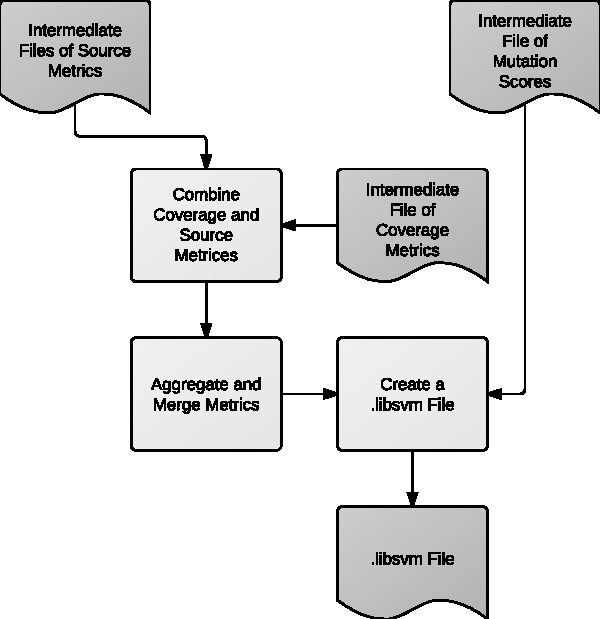
\includegraphics[width=5.25cm]{figures/process_part2.pdf}
    \end{minipage}
  \end{figure}
}

\subsubsection{.libsvm File}
\frame{\frametitle{.libsvm File}
  \begin{center}
    \begin{minipage}{6cm}
      \scriptsize
      \lstinputlisting{listings/libsvm_example.libsvm}
    \end{minipage}
  \end{center}
  \begin{minipage}{\linewidth}
    \begin{itemize}
      \item \texttt{LIBSVM}\footnote{\tiny{\url{csie.ntu.edu.tw/~cjlin/libsvm/}}} is a SVM library that requires a \alert{specific} file format for training and prediction
      \begin{itemize}
        \item \texttt{category attribute\_1:value attribute\_2:value \ldots}
      \end{itemize}
      \item We have \alert{class} and \alert{method} \texttt{.libsvm} file for predicting and training
    \end{itemize}
  \end{minipage}
}

\section{Results}
\frame{
  \setcounter{tocdepth}{2}
  \tableofcontents[currentsection,hideothersubsections]
}

\subsection{Case Study -- JGAP}
\frame{\frametitle{Case Study -- JGAP}
  \begin{minipage}{\linewidth}
    \begin{itemize}
      \item We present \alert{initial results} on an open source project -- JGAP (Java Genetic Algorithm Package).
      \item JGAP \alert{source code} has 28975 SLOC, 3017 methods, 415 classes.
      \item JGAP \alert{test code} has 19556 SLOC, 1626 methods, 180 classes.
      \item In total JGAP has 1412\footnote{\tiny{JGAP has 1412 JUnit test cases in total, however 25 of the tests caused errors in the \texttt{Javalanche} tool and were removed.}} \alert{JUnit test cases}.
    \end{itemize}
  \end{minipage}
}

\subsubsection{JGAP -- Class Mutation Score Distribution}
\frame{\frametitle{JGAP -- Class Mutation Score Distribution}

  \begin{figure}
    \centering
    \begin{tikzpicture}
    \begin{axis}[
        xtick={0, 25, 50, 75, 100},
        ytick={0, 2, 4, 6, 8, 10, 12, 14, 16},
        bar width=1,
        ymajorgrids=true,
        xlabel=Mutation Score (\%),
        ylabel=\# of Classes,
        width=\linewidth,
        height=6.0cm]
        \addplot[ybar,fill=black] file {plots/class_distribution.txt};
    \end{axis}
    \end{tikzpicture}
  \end{figure}

  \begin{itemize}
    \item Collected \alert{127 class-level} data points.
  \end{itemize}
}

\subsubsection{JGAP -- Method Mutation Score Distribution}
\frame{\frametitle{JGAP -- Method Mutation Score Distribution}

  \begin{figure}
    \centering
    \begin{tikzpicture}
    \begin{axis}[
        xtick={0, 25, 50, 75, 100},
        ytick={0, 20, 40, 60, 80, 100, 120, 140, 160, 180, 200, 220},
        bar width=1,
        ymajorgrids=true,
        xlabel=Mutation Score (\%),
        ylabel=\# of Methods,
        width=\linewidth,
        height=6.0cm]
        \addplot[ybar,fill=black] file {plots/method_distribution.txt};
    \end{axis}
    \end{tikzpicture}
  \end{figure}

  \begin{itemize}
    \item Collected \alert{695 method-level} data points.
  \end{itemize}
}

\subsubsection{JGAP -- Prediction Categories}
\frame{\frametitle{JGAP -- Prediction Categories}
  \begin{table}
    \centering
    \rowcolors{2}{gray!30}{gray!20}
    \begin{tabular}{|l|r|r|}
      \hline
      \rowcolor[RGB]{169,196,223}
      \textbf{Category} & \textbf{Class Mutation Score} & \textbf{Method Mutation Score} \\
      \hline low & 0.00\% -- 62.75\% & 0.00\% -- 66.66\% \\
      \hline medium & 62.75\% -- 83.25\% & 66.66\% -- 90.90\% \\
      \hline high & 83.25\% -- 100.00\% & 90.90\% -- 100.00\% \\
      \hline
    \end{tabular}
  \end{table}

  \begin{itemize}
    \item These mutation score ranges were selected to \alert{evenly distribute} the training data points across categories.
  \end{itemize}
}

\subsubsection{JGAP -- Cross Validation Accuracy}
\frame{\frametitle{JGAP -- Cross Validation Accuracy}
  \begin{table}
    \centering
    \rowcolors{2}{gray!30}{gray!20}
    \begin{tabular}{|l|r|r|}
      \hline
      \rowcolor[RGB]{169,196,223}
      \textbf{Set} & \textbf{Class Accuracy} & \textbf{Method Accuracy} \\
      \hline Source Metrics & 53.54\% & 48.77\% \\
      \hline Coverage Metrics & 49.61\% & 47.63\% \\
      \hline Sum/Avg Test Metrics & 45.67\% & 49.78\% \\
      \hline Sum/Avg Source Metrics & 54.33\% & 33.96\% \\
      \hline \textbf{All Metrics} & \textbf{58.27\%} & \textbf{54.82\%} \\
      \hline
    \end{tabular}
  \end{table}

  \begin{itemize}
    \item This validates our initial intuition that \alert{we need both source code and test suite metrics} to predict mutation score
  \end{itemize}
}

\section{Future Work}
\frame{
  \setcounter{tocdepth}{2}
  \tableofcontents[currentsection,hideothersubsections]
}

\subsection{More Attributes for Feature Data}
\frame{\frametitle{More Attributes for Feature Data}
  \begin{itemize}
    \item We are now considering \alert{new attributes} for feature data:
    \begin{itemize}
      \item \alert{Number of Tests Cases} for each source code unit.
      \item \alert{Number of Mutant Types} for each source code unit.
      \item \alert{Number of Total Mutants} for each source code unit.
    \end{itemize}
    \item We also want to \alert{optimize} the current set of attributes
  \end{itemize}
}

\subsection{More Data, More Questions}
\frame{\frametitle{More Data, More Questions}
  \begin{table}
    \centering
    \rowcolors{2}{gray!30}{gray!20}
    \begin{tabular}{|l|r|r|r|}
      \hline
      \rowcolor[RGB]{169,196,223}
      \textbf{Program} & \textbf{SLOC} & \textbf{Test SLOC} & \textbf{Test Cases} \\
      \hline jgap (3.6.1) & 28975 & 19694 & 1355 \\
      \hline joda-time (2.0) & 27139 & 51428 & 3866 \\
      \hline commons-lang (3.1) & 19499 & 33332 & 2050 \\
      \hline logback-core (1.0.3) & 12118 & 8145 & 286 \\
      \hline openfast (1.1.0) & 11646 & 5587 & 322 \\
      \hline joda-primitives (1.0) & 11157 & 6989 & 1810 \\
      \hline jsoup (1.6.2) & 10949 & 2883 & 319 \\
      \hline barbecue (1.5-beta1) & 4837 & 2910 & 225 \\
      \hline
    \end{tabular}
  \end{table}

  \begin{itemize}
    \item In general can we \alert{predict within projects?}
  \end{itemize}
}

\subsubsection{More Data, More Questions}
\frame{\frametitle{More Data, More Questions}
  \begin{table}
    \centering
    \rowcolors{2}{gray!30}{gray!20}
    \begin{tabular}{|l|r|r|r|}
      \hline
      \rowcolor[RGB]{169,196,223}
      \textbf{Program} & \textbf{SLOC} & \textbf{Test SLOC} & \textbf{Test Cases} \\
      \hline jgap (3.6.1) & 28975 & 19694 & 1355 \\
      \hline joda-time (2.0) & 27139 & 51428 & 3866 \\
      \hline commons-lang (3.1) & 19499 & 33332 & 2050 \\
      \hline logback-core (1.0.3) & 12118 & 8145 & 286 \\
      \hline openfast (1.1.0) & 11646 & 5587 & 322 \\
      \hline joda-primitives (1.0) & 11157 & 6989 & 1810 \\
      \hline jsoup (1.6.2) & 10949 & 2883 & 319 \\
      \hline barbecue (1.5-beta1) & 4837 & 2910 & 225 \\
      \hline
    \end{tabular}
  \end{table}

  \begin{itemize}
    \item Can we \alert{predict across projects?}
  \end{itemize}
}

% Ending slide is title page again
\section*{}
\frame{\titlepage}

\end{document}
